\documentclass[12pt]{article} \usepackage[utf8]{inputenc}
\usepackage{graphicx}
\usepackage{multirow}
\usepackage{hhline}
\usepackage{booktabs}
\usepackage{vmargin} %cambia el margen
\usepackage{amsmath, amsthm}
\usepackage{amsfonts}
\usepackage{float}
\usepackage{listings}
\usepackage{algorithm} % http://ctan.org/pkg/algorithms
\usepackage{algpseudocode} % http://ctan.org/pkg/algorithmicx
\usepackage{biblatex}

\bibliography{bibliography}

\renewcommand{\contentsname}{Índice}

\usepackage[hidelinks]{hyperref}

\title{
  Historia de las Matemáticas\\
  \large Historia de los algoritmos inspirados en la evolución:
  Algoritmos Genéticos, Programación Evolutiva, Estrategias de
  Evolución y Programación Genética.  }

\author{
  Francisco Luque Sánchez \\
  Ignacio Mas Mesa \\
  Miguel Morales Castillo \\
  María del Mar Ruiz Martín \\
}

\begin{document}
\maketitle
\begin{center}
  
\includegraphics[scale=0.35]{escudo.png}
\end{center}

\newpage

\tableofcontents % para generar el índice de contenidos

\pagebreak

\section{Introducción}

Las metaheurísticas son una clase de estrategias de resolución de
problemas que aparecieron en los años 50. Este tipo de algoritmos se
inspiran en procesos naturales, físicos o sociales para intentar
resolver problemas, usualmente de optimización, cuando el espacio de
soluciones es demasiado amplio para ser estudiado por métodos
tradicionales.\\

En este trabajo abordaremos, desde una perspectiva histórica, el
origen, evolución y estado actual de este tipo de técnicas, así como
ejemplos prácticos de aplicación. En particular, incidiremos sobre una
clase importante de metaheurísticas, las cuales se inspiran en el
proceso natural de la evolución. Dentro de este grupo se engloban
cuatro enfoques principales, que son los algoritmos genéticos, la
programación evolutiva, la programación genética y las estatregias
de evolución.\\

\section{Metaheurísticas}

Las metaheurísticas aparecieron en los años 50 como respuesta a los
problemas de optimización. Hasta ese momento, los ordenadores habían
sido utilizados como herramientas de ayuda al cálculo, pero no se
habían pensado como máquinas capaces de resolver problemas más
complejos. Cuando se intentaron implementar técnicas de optimización
clásica para resolver problemas de búsqueda (derivación de funciones
para el cálculo de extremos locales), se observó que para muchos
problemas este enfoque no era suficiente. Uno de los problemas que
surgió fue que las funciones a optimizar tenían muchos extremos
locales, infinitos en algunos casos. También se encontraron problemas
en los que las funciones a optimizar no eran derivables, por lo que el
enfoque clásico no podía
ser aplicado.\\

Empezaron a aparecer entonces intentos de resolución de problemas de
este tipo con estrategias distintas. El primer ejemplo de este tipo de
estrategias vino en 1951, con un método de aproximación estocástica.
Este método, creado por Herbert Robins y Sutton Monro, trataba de
encontrar extremos de una función utilizando un método de aproximación
por pasos que depende de una variable aleatoria. Así se puede buscar
el mínimo de una función sin tener que buscar la derivada de la misma.\\

Posteriormente, apoyándose en los trabajos de Robbins y Monro,
empezaron a aparecer los métodos de búsqueda local. Estos enfoques
consisten en tratar de buscar una solución al problema por medio de
evaluaciones de la función objetivo (función que tratamos de
maximizar). El primer método desarrollado en esta línea fue propuesto
por L. A. Rastrigin, que propuso el algoritmo conocido como
\textit{random search}. Consiste en comenzar evaluando la función
objetivo en un punto aleatorio del espacio de soluciones, y tras esto,
mientras no se haya alcanzado un criterio de parada (se hayan
terminado el número de iteraciones fijadas para el algoritmo, o se
haya alcanzado una cota para la solución establecida de antemano), se
siguen evaluando puntos en un vecindario cercano a la solución actual,
por medio de introducir un cambio aleatorio en la solución sobre la
que trabajamos, hasta que encontremos una solución que nos dé mejores
resultados que la que teníamos hasta el momento. Una vez encontrada
dicha solución más satisfactoria, se descarta la solución antigua
y se empieza a trabajar con la nueva.\\

Este enfoque se consideró interesante durante varios años, ya que
permitía encontrar soluciones razonablemente buenas a problemas de
optimización sencillos, pero que no podían resolverse con técnicas
clásicas de optimización.\\

Estas primeras aproximaciones, aunque todavía eran simples y no
obtenían buenos resultados, llamaron la atención de gran parte de la
comunidad, y empezaron a diseñarse estrategias más sofisticadas para
la resolución de problemas de este tipo. Las premisas de las que se
partían eran las siguientes:

\begin{itemize}
\item Se trataban de resolver problemas complejos, en los que el uso
  de técnicas clásicas quedaba descartado.
\item El espacio de soluciones era amplio, por lo que no podía
  estudiarse por completo.
\item No preocupa tanto la obtención de la solución óptima, si no que
  se adquiere un compromiso entre la bondad de la solución obtenida y
  el tiempo necesario para encontrar dicha solución.
\end{itemize}

A pesar de que estas premisas no fueron consensuadas hasta mediados de
los años ochenta, cuando se acuñó el término \textit{metaheurística}
por Fred W. Glover, las nombramos aquí porque suponen un punto de
partida importante para entender cómo se ha desarrollado esta rama.\\

Volviendo a los primeros pasos que se dieron en el campo, tras los
algoritmos de búsqueda local de principios de los años 60, en el año
1966 aparece el primer conjunto de algoritmos dentro de lo que se
conoce como computación evolutiva. La computación evolutiva es el
conjunto de estrategias que se basan en los principios de la evolución
darwiniana para desarrollar estrategias de resolución de problemas de
optimización. Es sobre este tipo de estrategias sobre las que
incidiremos durante el resto del trabajo. A modo de resumen, la
programación evolutiva, que es este primer conjunto de estrategias de
las que hablamos, fue descrita y desarrollada en un principio por
Lawrence J. Fogel. Aunque los primeros trabajos en los que se aplica
esta técnica son de principios de los 60, hasta el 66 no publicó Fogel
su artículo \textit{Artificial Intelligence Through Simulated
  Evolution}.  Se basa en una población de soluciones que mutan para
generar soluciones nuevas, las cuales entran en competencia con las
antiguas, de forma que sobreviven sólo las mejores soluciones
contempladas.\\

Este enfoque resulta novedoso en el punto en el que ahora no se tiene
una única solución que se modifica para explorar el espacio de
soluciones, si no que se tienen distintas soluciones repartidas, a
priori aleatoriamente, por todo el espacio de búsqueda, evitándose así
uno de los primeros problemas que se detectaron en algoritmos previos,
que era el atasco del algoritmo en óptimos locales, que impedían
encontrar soluciones mejores que se encontrasen a cierta distancia.\\

Dentro de la rama de la computación evolutiva, aparecen en Berlín de
forma prácticamente simultánea (con un par de años de diferencia) lo
que se conocen como estrategias de evolución. Desarrolladas por
Rechenberg y Schwefel, tienen un funcionamiento similar a la
programación evolutiva, aunque con ciertas diferencias que
concretaremos más adelante.\\

Tras estas aproximaciones, aparece en Míchigan en el año 1975 el
paradigma más extendido dentro de la computación evolutiva. Se trata
de los algoritmos genéticos, desarrollados y descritos por John H.
Holland. En esta estrategia se introduce el concepto de cruce entre
soluciones, en imitación al apareamiento entre especies animales.
Realmente, Holland comenzó a trabajar en el tema en los años 60, haciendo
su primera publicación al respecto en el año 1962, pero no es hasta el
1975 cuando se populariza su uso, año en el que el propio Holland publica
su libro \textit{Adaptation in Natural an Artificial Systems}.\\

En años posteriores, a principios de los 80, aparecen nuevos modelos,
que cambian el enfoque de los años anteriores, y empiezan a buscar
otras inspiraciones en procesos físicos para crear metaheurísticas.
Aparecen así ejemplos como \textit{Simulated annealing}, propuesto por
S. Kirkpatrick en 1983, que mejora el comportamiento de las búsquedas
locales introduciendo una probabilidad de avanzar hacia peores
soluciones, para intentar salir de óptimos locales. Esta probabilidad
va descendiendo a medida que avanza el algoritmo, de forma que al
principio la probabilidad de empeorar la solución es alta, lo que
aumenta la capacidad de exploración del espacio de soluciones del
algoritmo, y al final es pequeña, para intentar refinar todo lo
posible la buena solución encontrada. Este algoritmo imita el proceso
de enfriamiento de los metales fundidos, y la creación de las
estructuras cristalinas que se producen en el proceso. Cuando el metal
está caliente, la probabilidad de que se rompan las conexiones entre
las partículas del metal es más alta, llevando el material a un estado
más inestable (metáfora con el desplazamiento a peores soluciones en
primeras etapas del algoritmo), mientras que cuando se va enfriando,
se van creando más enlaces, para llevar al material a un estado
estable (búsqueda de mejores soluciones al final del algoritmo).\\

A mediados de los 80, concretamente en 1986, aparece otro avance
dentro del campo de las búsquedas locales. Fred W. Glover diseña la
búsqueda tabú, que funciona de la misma forma que las búsquedas
locales, pero permitiendo el avance hacia peores soluciones. Además,
como novedad incorpora una lista de \textit{soluciones tabú}, que son
soluciones evaluadas en las últimas iteraciones del algoritmo. Esta
lista sirve para evitar que el algoritmo retroceda hacia soluciones
anteriormente visitadas, de forma que no se pierdan iteraciones
del mismo sin sentido.\\

Tras estos avances, se intenta ahora hibridar los algoritmos obtenidos
hasta el momento para conseguir soluciones todavía mejores. Aparece
entonces el concepto de algoritmo memético, propuesto por Pablo
Moscato en el Instituto Tecnológico de Calfornia (Caltech) en
1989. Esta metodología trata de unir los algoritmos genéticos con los
algoritmos de búsqueda local. Consiste en ejecutar un algoritmo
genético de los anteriormente explicados, y cada cierto número de
generaciones (nombre con el que se conoce a las iteraciones de un
algoritmo genético) aplicar una búsqueda local sobre ciertos
individuos de la población, con el fin
de mejorar la solución que representan.\\

Tras este desarrollo, empiezan a aparecer algoritmos que se inspiran
en procesos biológicos, que se conocen como algoritmos bioinspirados.
En este sentido, aparece en 1992 el algoritmo de colonia de hormigas,
que simula la organización de un hormiguero, y la cooperación entre
hormigas para encontrar comida. Es ampliamente utilizado actualmente
para la búsqueda de caminos más cortos cuando se han de visitar un
conjunto ciudades (lo que se conoce como problema del viajante de
comercio).\\

Finalmente, ante la gran diversidad de algoritmos que aparecieron para
resolver problemas de optimización, los investigadores en el área
empezaron a preguntarse si existe un único algoritmo que sea capaz de
resolver correctamente cualquier clase de problemas. Durante varios
años se estuvo investigando en este área, hasta que en 1997 se
enunciaron y demostraron (por parte del matemático David Wolpert y el
informático William Macready) los \textit{Non free lunch theorems for
  optimization}. Dichos teoremas sostienen que ``en media, los
resultados obtenidos por dos algoritmos de optimización sobre todas
las clases de problemas posibles son equivalentes''. Esto viene a
decir que, si un algoritmo tiene un mejor comportamiento para una
clase de problemas, se verá perjudicado al intentar resolver problemas
de otro tipo. Esto viene a justificar que se siga investigando en este
área.

\section{Algoritmos genéticos}

Los algoritmos genéticos pertenecen a la amplia familia de los
algoritmos evolutivos.  Sin embargo, a diferencia de la mayoría de
algoritmos evolutivos, que surgen con la finalidad de resolver
problemas de simulación para ingeniería y biología o para problemas de
optimización, su origen es sustancialmente diferente. A principios de
los años 60, John Henry Holland, profesor de psicología, ingeniería
eléctrica y ciencias de la computación en la universidad de Míchigan,
comienza a desarrollar lo que él llama los algoritmos
genéticos. Holland propone estos algoritmos en su búsqueda por
comprender la evolución de una población, y de forma más general, de
encontrar los criterios seguidos por los sistemas adaptativos. Publica
así en 1962 un estudio sobre el tema, estudio que
se considerará el nacimiento de los algoritmos genéticos.\\

Holland inicialmente propone un sistema adaptativo formado por una
población de cromosomas que irán evolucionando de forma que las
futuras generaciones tiendan a ser mejores. Para ello, contará con
cromosomas, que serán cadenas binarias, donde cada uno de sus
elementos será llamado gen. A partir de una población inicial, los
cromosomas interactuarán de forma iterativa dando lugar a nuevas
generaciones. El proceso iterativo contará con las siguientes fases:
en primer lugar se realiza una selección de individuos en nuestra
población para reproducirse. A continuación se aplica un operador de
cruce entre los padres, de forma que se obtengan descendientes
similares a ambos. Se pasa a aplicar una serie de modificaciones
aleatorias a algunos, o a todos, los descendientes obtenidos. En un
proceso conocido como mutación. A continuación se aplicará el operador
de inversión, que consiste en tomar una subcadena del cromosoma y
sustituirla por su inversa. Finalmente se somete a la población
anterior, junto a la descendencia obtenida a un proceso de selección,
en el que se seleccionarán los mejores individuos según una función
fitness, y éstos pasarán
a formar la nueva generación.\\

Holland entendía esta función fitness como una medida de la capacidad
de competición e innovación de los individuos para dinámicamente
responder ante cambios no predecibles del ambiente. Con esta
formulación de los algoritmos genéticos, Holland fue el primero en
introducir explícitamente las nociones de cruce, o cualquier otro tipo
de operadores de recombinación
en el ámbito de los algoritmos evolutivos.\\

En los próximos años, surgen figuras como Bagley, cuya tesis trata
sobre la aplicación de los algoritmos genéticos sobre la función de
evaluación en programas que juegan a juegos, o la tesis de Cavicchio
(1970) en la que trata los algoritmos genéticos desde una perspectiva
de búsqueda adaptativa.  Introduce además el concepto de elitismo, con
el que cada generación mantendrá la mejor solución obtenida hasta el
momento, y operadores de mutación que se
adaptan a lo largo de las iteraciones según las necesidades de cada generación.\\

A pesar de las figuras anteriores y algunas más, durante los años
sesenta el principal desarrollo y estudio de los algoritmos genéticos
se centra en la universidad de Míchigan, con John Holland y sus
estudiantes. Será durante estos años cuando Holland, junto con algunos
alumnos de doctorado desarrollará una
función fitness con la que predecir la calidad de cada generación.\\

En 1972 destaca la tesis de Frantz, en la que propone nuevas técnicas
de cruce,
con lo que se conoce como operadores de cruce multipuntos.\\



En 1975 se produce el evento más importante de la historia de los
algoritmos genéticos cuando John Holland publica su libro ``Adaptation
in Natural and Artificial Systems'' en el que establece la estructura
de los algoritmos genéticos y presenta un estudio matemático de los
fundamentos teóricos de los mismos. Esto último supone un gran avance
en el campo de los algoritmos evolutivos, puesto que es la primera vez
que se estudia teóricamente el
comportamiento de algún algoritmo evolutivo.\\


En su libro John Holland mantiene la estructura original que propuso
en 1962, pero añade la noción de ``esquemas''. Un esquema será
simplemente un patrón presente en la estructura de los cromosomas. A
partir de los esquemas Holland establecía una medida de bondad de la
generación actual a partir de los valores fitness obtenidos para cada
esquema, donde entendía el valor fiteness de un esquema como la media
de los valores obtenidos por cada cromosoma de la población que
cumpliese el esquema en cuestión. Con esta medida se pretendía guiar
el proceso
de evolución de la población. \\

A partir de lo anterior introdujo una formalización para predecir la
calidad de la siguiente generación a partir de lo que se conoció como
el Teorema de los
esquemas de Holland.\\



También en 1975, Kenneth De Jong, estudiante de doctorado de Holland,
presenta su tesis doctoral, que será el primer estudio del uso de
algoritmos genéticos para resolver problemas de optimización. Con el
trabajo de Kenneth se pone de manifiesto la utilidad práctica de los
algoritmos genéticos. Además establece un estándar a seguir con los
mismos, y durante años cualquier estudio de calidad sobre algoritmos
genéticos seguía las pautas marcadas por Kenneth y presentaba
los benchmarks presentes en su tesis.\\

En dicha tesis, De Jong no solo estudia teóricamente el comportamiento
de los algoritmos genéticos, sino que también los estudia desde un
punto de vista experimental. Además, pone de manifiesto el potencial
que presentan los algoritmos genéticos para resolver problemas de
optimización desde un punto de vista teórico,
potencial que ya había sugerido anteriormente Sampson.\\

Tras estas dos principales publicaciones, aumentan en los años 70 y 80
las investigaciones sobre los algoritmos genéticos. Poco a poco los
algoritmos genéticos van cogiendo fuerza en el terreno científico y
surge una comunidad de estudios de los mismos.  Aumenta también la
aplicación de los mismos, que empiezan a aplicarse en campos de
ingeniería y optimización sobre funciones con domino en los enteros.\\

A mediados de los 70 en otras universidades comienzan a estudiar los
algoritmos genéticos, y comienzan a aparecer múltiples tesis
doctorales sobre los mismos, de las que se podrían destacar las de
Bethke, Booker, y Goldberg. Sin embargo, el desarrollo de los
algoritrmos genéticos continúa siendo muy lento, ya que la comunidad
de la Inteligencia Artificial aún era excéptica ante los mismos y se
centra en el desarrollo de otras técnicas novedosas
y de gran funcionalidad como el nacimiento del perceptrón.\\

En el verano de 1976, investigadores de diversas universidades, entre
ellas las de Michigan, Pitsburg o Alberta, organizaron una conferencia
sobre sistemas adaptativos en Ann Arbor, Míchigan. Apenas participaron
20 investigadores, pero supuso la puesta en contacto de diversos
científicos que trabajaban en el área de los algoritmos
genéticos. Durante los siguientes años siguieron repitiendo el
evento. Y en 1981 Holland, De Jong y Sampson fundan ``An
Interdisciplinary Workshop in Adaptive Systems'' en la universida de Míchigan.\\


Hasta los años 80 el desarrollo de los algoritmos genéticos había
seguido un enfoque muy teórico, pero el aumento del interés de la
comunidad científica en los mismos desemboca en que a mediados de los
años 80 se organice
en Pittsburgh, Pensilvania, la Primera Conferencia Internacional de Algoritmos Genéticos.\\

En esta conferencia, con 75 participantes, se discutieron temas tanto
teóricos como prácticos de los algoritmos genéticos. El éxito de la
conferencia fue tal que acordaron repetirla con
carácter bianual.\\

A partir de estas conferencias comienzan a surgir numerosos libros
sobre el tema. Cabe destacar el publicado por Golsberg (1987), puesto
que presenta una visión clara y precisa de los algoritmos genéticos en
un tono sencillo, fácil de entender para cualquier persona aunque no
fuera experta en el tema. Esto supone una amplia
difusión de los algoritmos genéticos.\\


El gran crecimiento de la comunidad desembocó en la creación de la
Sociedad Internacional de Algoritmos Genéticos (ISGA) en 1989. A
partir de entonces el desarrollo de los algoritmos genéticos
presenta un crecimiento rápido y desordenado, sin seguir ningún
estándar, y utilizados también para optimizar problemas de naturaleza
real. En consecuencia, los 90 fueron un periodo de tremendo
crecimiento y diversidad del área de los algoritmos genéticos. \\


Conforme surgen nuevos estudios de los algoritmos genéticos, se
comprueba que las características que Holland establecía en su libro
``Adaptation in Natural and Artificial Systems'' como deseables en un
algoritmo genético, no concuerdan con los experimentos obtenidos. Esto
se debe principalmente a que, por la reducida capacidad de cálculo que
se tenía, los experimentos realizados por Holland previos a sus
conclusiones habían sido con muestras muy pequeñas y tamaños de
poblaciones demasiado
pequeñas, dando lugar a que los resultados no fuesen fiables. \\

Sin embargo, a pesar de la mala predicción de las características
estimadas por Holland de un algoritmo genético, el uso de los esquemas
como fundamento teórico del buen funcionamiento de los
algorítmos genéticos ha sido ampliamente aceptado hasta hace poco.\\


Lo cierto es que, más allá de la descripción dada en ``Adaptation in
Natural and Artificial Systems'' no existe una definición rigurosa de
qué es un algoritmo genético que sea aceptada por la comunidad de los
algoritmos evolutivos, y muchas veces la frontera entre estos
algoritmos y otros evolutivos es
realmente débil. \\

Sin embargo, la mayoría de los algoritmos hoy catalogados como
algoritmos genéticos coinciden en los siguiente elementos: se cuenta
con una población de cromosomas, que a partir de una función fitness
que se pretende optimizar son sometidos a los operadores de selección,
cruce, mutación y reemplazamiento de forma iterativa buscando
optimizar el valor de dicha función fitness.  Podemos notar que el
operador de inversión introducido por Holland ha desaparecido del
panorama actual, ya que recibió duras críticas debido a que sus
ventajas, en caso de existir, no han
sido establecidas o explicadas.\\


\section{Programación evolutiva}

Uno de los primeros enfoques que se tomaron dentro del ámbito de la
computación evolutiva fue el de la programación evolutiva. Fue
propuesto por Lawrence J. Fogel, un estudiante de la Universidad de
Nueva York y doctorado por la Universidad de California. Comenzó
trabajando como ingeniero aeroespacial en \textit{General Dynamics}
tras terminar la carrera en ingeniería eléctrica. Tras esto, sirvió
como asistente del Director Asociado en la \textit{National Science
  Foundation}, donde estuvo trabajando en modelos matemáticos para
predecir el impacto económico que tendría la inversión en
investigación científica.  Dichos estudios fueron aplicados en varias
agencias gubernamentales, como el Departamento de Defensa, la
Administración Nacional Espacial y Aeronáutica, el Departamento de
Salud, o la Administración Educativa. Este trabajo multidisciplinar
motivó el interés de Fogel en diversas áreas como la cibernética o la
biotecnología, y lo llevó a la hipótesis de que la simulación de la
evolución en un ordenador podía ser utilizada para generar
inteligencia artificial.\\

Todos estos razonamientos fueron puestos en práctica tras su vuelta a
\textit{General Dynamic}, donde comenzó a explorar la programación
evolutiva en la predicción de series temporales. Tras estos trabajos,
publicó su tesis en la Universidad de California, como hemos
mencionado antes, en la que comenzó a hablar del término programación
evolutiva y su utilidad para la resolución de problemas de
optimización y búsqueda. Dicha tesis tuvo lugar en el año 1964, y es
la fecha en la que se considera que se especificó y desarolló la
técnica.\\

Tras esto, en 1965, abandonó su puesto en \textit{General Dynamics}
para fundar su propia empresa, \textit{Decision Science, Inc.}, que
estaba enfocada a la aplicación de la programación evolutiva para la
resolución de problemas reales, específicamente en las áreas de
simulación por ordenador, predicción y control de sistemas. Dicha
empresa fue pionera en ser ideada específicamente para aplicar la
computación evolutica para resolver problemas reales, y no como mera
investigación dentro de la materia.\\

Las bases sobre las que trabajó Fogel son las siguientes. Se trataba
de predecir el comportamiento de un entorno cambiante dependiente del
tiempo (serie temporal), para intentar tomar acciones en función del
comportamiento esperado del sistema. Se codificaba entonces el estado
del sistema utilizando una secuencia de símbolos cogidos de un
alfabeto finito, y dicha secuencia se lee con un autómata finito, que
produce una salida.\\

La propuesta de Fogel es entonces tener un conjunto de autómatas
finitos, que forman la población de soluciones. Para cada autómata
finito, se evalúa su capacidad de predicción utilizando la salida que
utiliza para la cadena de entrada. Se define una función de adecuación
o \textit{fitness}, que mide el grado de corrección en la predicción
del autómata en ese entorno.\\

Tras tener la población de padres generados de forma aleatoria y
evaluados, se genera un población de hijos ``mutando'' la población de
padres. Cada padre genera un único hijo. Según Fogel, existen cinco
tipos de mutaciones posibles, atendiendo a la descripción de autómata
finito:

\begin{enumerate}
\item Cambiar un símbolo de salida
\item Cambiar una transición de estado
\item Añadir un estado
\item Eliminar un estado
\item Cambiar el estado inicial
\end{enumerate}

Propuso mutaciones más fuertes más adelante, pero no llegó a
implementarlas. Las mutaciones que se producían eran seleccionadas
respecto de una variable aleatoria. Una vez producida la población de
hijos por mutación, se evaluaban de la misma manera que los padres,
Tras esto, entraban en competición los padres con los hijos de forma
que sólo permanecían en la población para generar la siguiente prole
la mitad mejor de los individuos. De esta forma, el tamaño de la
población de padres permanece constante durante todo el algoritmo.
Este proceso de mejora de las predicciones por la población se repetía
hasta que era necesario generar un nuevo símbolo (había que hacer una
predicción nueva). En ese momento, se utilizaba toda la población para
predecir el siguiente símbolo (se tomaba como siguiente símbolo el
símbolo predecido en más ocasiones por la población), se introducía
dicho símbolo en la cadena de entrada, y la nueva cadena se seguía
utilizando para entrenar a la población.\\

La propuesta de Fogel fue utilizada para la resolución de multitud de
problemas, entre los que destacan problemas de predicción y control
automático, llevados a cabo por el propio Fogel, o reconocimiento de
patrones y máquinas que juegan a juegos, trabajos realizados por
Huntsinger en 1969 o Burgin ese mismo año.\\

Tras aplicarse este enfoque durante más de una década, a mediados de
los años 80 comenzaron a proponerse nuevas estructuras de datos que
podían ser interpretadas como individuos de una población, y por tanto
podían ser utilizadas para algoritmos de programación
evolutiva. Aparecieron así algoritmos que hacían uso de listas
ordenadas para resolver el problema del viajante de comercio, o
vectores de variables reales que permitían la optimización de
funciones. Estos nuevos esfuerzos llevaron a la aplicación de la
programación evolutiva para la planificación de rutas (trabajos de
Fogel en 1988), soluciones al problema de la mochila (Fogel, 1989), o
a métodos de entrenamiento y ajuste de parámetros de redes neuronales.\\

Paralelamente a estos avances, Fogel comenzó a investigar también en
nuevos mecanismos para controlar el proceso de evolución por mutación
que sufrían los individuos. Llamó a este proceso
\textit{autoadaptación}.  Se dió cuenta de que un buen ajuste en la
forma de mutar que producía el algoritmo podía mejorar enormemente los
resultados obtenidos por el mismo. De esta forma, comenzó a probar
estrategias que cambiaban la probabilidad de que se produzcan
mutaciones en función del punto de ejecución del algoritmo en el que
nos encontremos (en función del número de iteraciones que se habían
producido ya, o que faltaban por producirse).\\

Ya en los años 90 se intentó dotar de importancia a esta estrategia de
resolución de problemas. Empezaron a organizarse entones conferencias
de carácter anual que versaban sobre programación evolutiva. Fruto de
estas conferencias aparecieron aplicaciones de la programación
evolutiva al campo de la robótica (trabajos de McDonnell y Andersen en
1992), y el diseño y entrenamiento de redes neuronales, trabajos
llevados a cabo por el propio Fogel.\\

De forma prácticamente simultánea a la aparición de estas
conferencias, comenzó el contacto de esta disciplina con la que se
explicará a continuación, que son las estrategias de evolución. Estas
dos áreas tienen grandes puntos en común, y algunos de los principales
investigadores en el área de las estrategias de evolución participaron
en las conferencias previamente mencionadas. Fueron especialmente
relevantes los trabajos de Thomas Bäck entre los años 1993 y
1995. Bäck, profesor en la Universidad de Leiden, es uno de los
principales exponentes de la computación evolutiva a día de hoy.\\

Después de la primera mitad de los 90, se diversificaron mucho los
esfuerzos en la aplicación de estas técnicas a la resolución de
problemas, apareciendo aplicaciones de tratamiento de imagen,
o el estudio de sistemas difusos. Finalmente, la aplicación que se
ha alzado como principal de la programación evolutiva es la del
entrenamiento de redes neuronales.

\section{Estrategias de evolución}

De forma casi paralela a la aparición de los \textbf{algoritmos
  genéticos} y la \textbf{programación evolutiva} en Estados Unidos,
se desarrollaron en la segunda mitad de la década de los 60 en
Alemania las \textbf{estrategias evolutivas} (\textit{evolution
  strategies}, ES). En 1964, tres estudiantes de la Technical University of
Berlin, viz.: Bienert, Rechenberg y Schwefel, se encontraron con un
problema de diseño durante sus estudios de tecnología aeroespacial. La
pieza a diseñar debía ser probada en una serie de experimentos en el
túnel de viento con el objetivo de minimizar su rozamiento. \\

Tras aplicar diversas técnicas \textit{clásicas} de análisis numérico a
estos efectos, como el gradiente descendente, los resultados obtenidos
fueron pobres, al menos lo suficiente como para tratar de explorar
otras posibilidades. En ese momento Rechenberg decidió aplicar
técnicas estocásticas usando dados para la generación de números
aleatorios. Así nació la primera versión de las estrategias
evolutivas, una $(1 + 1)$ ES en la notación actual, i.e.: en cada
paso se consideraba una única solución \textit{padre}, de la cual se
variaban aleatoriamente ciertas características. Una vez hecho esto,
se comparaba la versión modificada con la original y se conservaba la
mejor de ambas, continuando con el proceso mientras se considerara
conveniente. \\

Para comprobar la eficacia de esta nueva aproximación se trató de
encontrar el óptimo, en un problema en dos dimensiones, de un problema
similar al que se enfrentaban. Durante unas cuantas iteraciones el
proto-algoritmo se mantuvo encallado en un óptimo local, para
finalmente converger al óptimo global teórico. \\

Más tarde, Bienert construyó un robot para llevar a cabo estos
cálculos de forma automática; y Lihchtfu{\ss} aplicó con éxito esta técnica para
el diseño de una tubería. El resultado fue inesperado, pero claramente
mejor que los diseños conocidos hasta el momento. Asimismo, se empleó
para diseñar una tobera que debía propulsar agua a velocidades
supersónicas. Este experimento resultó especialmente interesante pues,
entre otros factores, se desconocía la longitud óptima de la
tobera. Para incluir esto en el espacio de búsqueda se emuló el
duplicado/eliminación de genes, de forma que se pudiera trabajar con un número
variable de parámetros indicando el diámetro de la tobera en distintos
puntos. \\

Sin embargo, pronto se descubrió que esta estrategia tenía sus
inconvenientes. En particular, las distribuciones binomiales usadas
hasta el momento producían, en muchas ocasiones, convergencia
prematura a óptimos locales que dejaban mucho que desear. Es por esto
que de ahí en adelante se adoptó como práctica común el empleo de
distribuciones normales en lugar de binomiales para la generación de
números aleatorios. \\

Posteriormente, Rechenberg elaboró su tesis en 1971 estudiando los
ratios de convergencia de las soluciones en distintos casos,
obteniendo la famosa \textit{regla del quinto} (\textit{$\frac 1 5$th
  rule}) y trató de optimizar el algoritmo aproximándolo más a lo que
ocurría en la naturaleza, considerando una \textit{población} de
soluciones en cada generación e introduciendo el paso de la
\textit{recombinación} de soluciones además de la mutación, dando
lugar a lo que, en la notación de Schwefel, se denominó $(\mu + 1)$ ES
($\mu$ padres, $1$ hijo). Nótese que este nuevo paso no habría sido posible en
las $(1 + 1)$ ES primigenias. \\

No obstante, aun esta modificación no fue suficiente en términos de
capacidad de adaptación, por lo que aparecieron las $(\mu + \lambda)$
y $(\mu, \lambda)$ ES, con $\mu$ padres y $\lambda$ descendientes en
cada generación. \\

\begin{description}
\item[$(\mu + \lambda)$] Se seleccionan los $\mu$
  mejores individuos de entre los $\mu$ padres y los $\lambda$
  descendientes de cada generación.
\item[$(\mu, \lambda)$] También se crean $\lambda$ descendientes en
  cada generación a partir de los $\mu$ padres. En este caso, sin
  embargo, los padres \textbf{no} pueden sobrevivir, seleccionándose
  los $\mu$ mejores descendientes de los $\lambda$
  considerados. Claramente, es necesario que $\lambda > \mu$. En el
  caso límite $\mu = \lambda$ todos los descendientes de cada
  generación se seleccionan como padres, sin importar su bondad, por
  lo que la población simplemente se dispersa aleatoriamente por el
  espacio de búsqueda.
\end{description}

Cabe destacar que, pese a los éxitos cosechados experimentalmente, los
inicios de esta disciplina fueron duros pues la comunidad científica
de la época se mostraba reticente a aceptar (creer) su versatilidad y
eficiencia por varios motivos.

\begin{itemize}
\item Durante la década de los 60 los métodos numéricos observaron un
  desarrollo inaudito, ganándose el respeto de los investigadores de
  la época y convirtiéndose incluso en \textit{buzzword}. Así, la
  necesidad de considerar otras técnicas era cuestionable,
  especialmente estas que no venían acompañadas de una justificación
  teórica en cuanto a su eficacia. Esto cambió más tarde tras diversos
  análisis por parte de Rechenberg, Schwefel y otros sobre su
  algoritmo.
\item Aun aceptando la posibilidad de que la $(1 + 1)$ ES fuera un
  artefacto útil en ciertos casos, la incorporación de las $(\mu +
  \lambda)$ ES no tuvo muy buena acogida. Por un lado, considerar $\mu >
  1$ individuos en la población se consideraba innecesario, pues
  simplemente aumentaba los tiempos de cálculo arrastrando individuos
  poco (menos) prometedores. Por otro, $\lambda > 1$ parecía no
  explotar inmediatamente el conocimiento obtenido en generaciones previas.
\end{itemize}

Si bien la crítica referida a los $\lambda > 1$ descendientes podía ser
rebatida gracias a la computación en paralelo de los vástagos, el
contraargumento no tenía mucho peso pues los ordenadores con
arquitecturas capaces de procesamiento en paralelo no existían ni se
los esperaba en el futuro próximo. \\

Finalmente, tras todos los cambios introducidos a lo largo de su
historia, la versión actual de una ES genérica puede verse resumida en la
siguiente figura:

\begin{figure}[H]
  \begin{algorithm}[H]
    \begin{algorithmic}[1]
      \label{ES-alg}
      \Procedure {ES}\,
      \State $g := 0$
      \State initialize $\left( P_p^{(0)} := \left\{ \left(y_m^{(0)},
            s_m^{(0)}, F(y_m^{(0)}) \right), m = 1, ..., \mu \right\}
      \right);$
      \Repeat

      \For {$l := 1$ \textbf{To} $\lambda$}
      \State $O_l :=$ marriage $\left( P_p^{(g)}, \rho \right);$
      \State $s_l :=$ s\_recombination $\left( O_l \right);$
      \State $y_l :=$ y\_recombination $\left( O_l \right);$
      \State $\tilde{s_l}$ := s\_mutation $\left( s_l \right);$
      \State $\tilde{y_l}$ := y\_mutation $\left( y_l, \tilde{s_l} \right);$
      \State $\tilde{F}_l := F(\tilde{y_l})$
      \EndFor

      \State $P_0^{(g)} := \left\{ \left( \tilde{y_l}, \tilde{s_l},
          \tilde{F_l} \right), l = 1, ..., \lambda \right\};$

      \If {selection\_type $ == (\mu, \lambda)$}
      \State $P_p^{(g+1)} := \mathrm{selection} \left( P_o^{(g)}, \mu \right);$
      \ElsIf {selection\_type $ == (\mu + \lambda)$}
      \State $P_p^{(g+1)} := \mathrm{selection} \left( P_o^{(g)}, P_p^{(g)} \mu \right);$
      \EndIf

      \State $g := g + 1$

      \Until termination condition
      \EndProcedure
    \end{algorithmic}
  \end{algorithm}
  \caption{Pseudocódigo del $\left( \mu / \rho \ \overset{+}{,} \ \lambda \right)$-ES \cite{beyer-es}}
\end{figure}

En la notación actual, las $(\mu / \rho \ \overset{+}{,} \ \lambda)$ ES consideran $\mu$ padres en cada generación, escogiéndose $\lambda$ subconjuntos de $\rho$ individuos para dar, cada uno de ellos, uno de los $\lambda$ descendientes. Como se había discutido previamente, en la versión ``$+$'' tanto los padres como la prole pueden pasar a la siguiente generación, mientras que en la versión ``,'' sólo los descendientes pueden sobrevivir. \\

La descripción del pseudocódigo del algoritmo es como sigue:

\begin{enumerate}
\item En la primera generación ($g = 0$) se inicializa la población de padres (de qué forma concreta dependerá de cada problema).
\item A continuación entramos en el bucle principal
  \begin{enumerate}
  \item Se comienza generando los descendientes de la generación actual. Cada iteración genera un nuevo vástago.
    \begin{enumerate}
    \item En primer lugar, el paso de la maridación (\textit{marriage}) selecciona una \textit{familia} de padres $O_l$ de tamaño $\rho$. Esta selección es completamente aleatoria, a diferencia de los algoritmos genéticos en los que se favorece la selección de los mejores padres.
    \item Más tarde le llega el turno a la recombinación, tanto de las características de las soluciones (\textit{object parameters}) como de las de la estrategia (\textit{strategy parameters}). De nuevo, cómo se recombine la información de cada padre dependerá de una implementación a otra y no existe una forma óptima.
    \item Por último, se mutan los \textit{strategy parameters} obtenidos de la recombinación y, sólo entonces, las características de la solución con los nuevos \textit{strategy parameters} obtenidos. Finalmente se calcula la bondad de la nueva solución obtenida mediante la función objetivo.
    \end{enumerate}
  \item Una vez generados todos los descendientes, se distingue entre el esquema de  selección $(\mu, \lambda)$ y $(\mu + \lambda)$:
    \begin{enumerate}
    \item En el primer caso se seleccionan los $\mu$ descendientes
    \item En el segundo caso se seleccionan los $\mu$ mejores individuos de entre los padres ($P_p^{(g)}$) y los descendientes ($P_o^{(g)}$).
    \end{enumerate}
  \item Para finalizar se actualiza la generación actual.
  \item El bucle principal se repetirá mientras no se alcance la condición de parada que, de nuevo, depende en gran medida de la casuística concreta del problema.
  \end{enumerate}
\end{enumerate}

Conviene notar que los mentados \textit{strategy parameters} constituyen la principal diferencia entre las estrategias evolutivas y los algoritmos genéticos u otras variantes de los algoritmos evolutivos. Estos controlan el tamaño de las mutaciones que sufre cada individuo, de forma que este tamaño también sea adaptativo, como una suerte de enfriamiento simulado implícito. Así, al recombinar padres para procrear un descendiente, no sólo se combinarán las características/parámetros propios del problema sino también los parámetros asociados a las mutaciones de los distintos factores; y, del mismo modo, las mutaciones también se aplicarán a los propios \textit{strategy parameters}. De este modo el propio algoritmo es capaz de autorregular lo que en otras aproximaciones a este tipo de técnicas suele convertirse en un arte más que una ciencia, es decir, el tamaño de las mutaciones. \\

\section{Programación genética}


\subsection{Introducción histórica}


La programación genética es un caso particular de algoritmos genéticos
usados para mejorar programas de ordenador de un modo automático.  La
población la componen programas de ordenador (individuos) que se
cruzan unos con otros, y al igual que ocurre con los algoritmos
genéticos, con el paso del tiempo, los mejores individuos sobreviven
y eventualmente evolucionan para mejorar. \\

La primera referencia que se tiene de evolucionar programas es
probablemente la de Alan Turing en la década de los 50. Sin embargo,
pasaron 30 años hasta que Richard Forsyth demostrara el éxito en la
evolución de pequeños programas, representados como árboles,
para mejorar la clasificación de las pruebas de una escena de crimen.\\

En 1988 John Koza, estudiante de John Holland, patentó un algoritmo
genético orientado a la evolución de programas, seguido de una
publicación en la International Joint Conference on Artificial
Inteligence. Koza ha sido el exponente principal de la programación
genética aplicando ésta a problemas complejos de búsqueda.
En la década de 1990, la programación genética se aplicó
principalmente para resolver problemas sencillos debido a su alto
coste computacional.\\

Recientemente la programación genética ha cobrado protagonismo debido
a los resultados positivos que ha mostrado en áreas como la computación
cuántica, ordenamiento y búsqueda gracias a la potencia de cómputo de
la que disponemos actualmente. Una de las grandes metas de la ciencia
de la computación es, dado un problema, que la máquina sea capaz de
construir un programa capaz de resolverlo, y la programación genética
muestra suficiente potencial para conseguirlo en un futuro.\\


\subsection {Creación de la población}

Cada individuo se representa mediante una estructura de árbol, donde
los nodos no terminales representan funciones cuyos hijos son los
parámetros que necesita la función como argumento, esto supone un
cambio respecto a los algoritmos genéticos donde los individuos se
representan mediante estructuras lineales como valores reales o
cadenas de bits.

\begin{figure}[H]
  \centering
  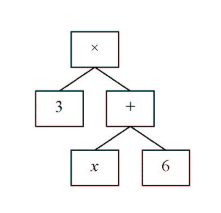
\includegraphics[width=0.4\textwidth]{individuo.PNG}
  \caption{Individuo que representa la función \(3\times(x+6)\).}
  \label{fig:dfd:1}
\end{figure}


La elección de los genes disponibles es una tarea importante
ya que una mala selección podría causar que no evolucione
la solución.\\

Una vez que los genes han sido seleccionados, se genera una
población de individuos de forma aleatoria y sin repetición
como ocurre con los algoritmos genéticos. Koza desarrolló
tres técnicas para ello: grow,full y ramped-half-and-half.


\subsubsection{Grow}

La población es creada eligiendo una profundidad máxima \(m\),
con esta técnica se crea un individuo nuevo cada vez con una
profundidad no mayor a \(m\),
el proceso se realiza de la siguiente forma:
\begin{itemize}
\item Desde la raíz , cada nodo se elige como función o terminal de
  forma aleatoria.
\item Si el nodo es terminal, se le asigna un nodo terminal de forma
  aleatoria
\item Si el nodo es una función, se le asigna una función de forma
  aleatoria y a ese nodo se le añaden tantos hijos como parámetros
  tenga la función elegida. Para cada hijo se repite el mismo proceso,
  a no ser que ya tenga profundidad \(m\),
  en ese caso para el hijo se selecciona un terminal aleatorio.
\end{itemize}

Esta estrategia genera individuos de profundidad variable no mayor que
\(m\) pero proporciona un rango de variedad muy amplio en la población.

\subsubsection{Full}

Esta estrategia, a diferencia de grow, garantiza que todos los
individuos tienen la misma profundidad, aunque el número de nodos es
variable. Aquí también se necesita especificar una profundidad \(m\),
y el proceso es el siguiente:\\

Partiendo de la raíz, cada nodo con una profundidad menor que \(m\)
, se convierte en una función aleatoria. Si el nodo tiene profundidad
\(m\) entonces se convierte en un terminal aleatorio. Todas las funciones
tienen un número de hijos igual a la cantidad de parámetros que necesitan
como argumento. Con esta estrategia te aseguras que todos los individuos
tienen una profundidad \(m\) aunque por contra la variación es menor
que con la estrategia grow.\\

\subsubsection{Ramped-half-and-half}

Se propone esta estrategia para aumentar la variación usando las dos
estrategias anteriores. Solo se especifica una profundidad máxima, y
se generan la mitad de los individuos usando el método grow, mientras
que la otra mitad se genera usando el método full, creando así una
población con una gran diversidad.

\subsection{Función Fitness}

Al igual que ocurre en los algoritmos genéticos, una vez que la
población esta inicializada, los individuos necesitan ser evaluados
para saber lo buenos o malos que son. La función fitness más
común es aquella que se adapte de forma más natural al problema que se
plantee. Un ejemplo sería el problema de clasificación donde la
función fitness más natural sería el número de aciertos.

\subsection{Operadores}

Análogamente a los algoritmos genéticos, la programación genética
cuenta con operadores de selección, cruce y mutación. Actualmente se
consideran otras operaciones como la edición, permutación o el
encapsulamiento, aunque la mayoría de ellas fueron ignoradas por Koza
en sus primeros trabajos.

\subsubsection{Selección}

Para la selección se utilizan los mecanismos habituales de los
algoritmos genéticos, en el caso de la programación genética, Koza
permitía que un 10\% de la población se pudiese reproducir además del
proceso de selección habitual. La función de selección es la encargada
de elegir que individuo se reproduce, cuya reproducción no es más que
elegir a ese individuo e introducir una copia de él mismo en la
población, si la función fitness es fija, la reproducción tiene un
efecto significativo en el tiempo ya que un individuo generado por
reproducción tendrá el mismo valor fitness que su padre.

\subsubsection{Cruce}

El proceso del operador de cruce es similar al de los algoritmos genéticos,
en este caso generamos aleatoriamente una arista a cada padre y se
intercambian los subárboles generando así dos hijos nuevos.\\

Algunas consideraciones a tener en cuenta pueden ser la de no efectuar
el cruce si la profundidad del árbol supera el máximo para evitar que
crezca indefinidamente. Otra consideración posible sería la de
incorporar criterios que penalicen en la función fitness una excesiva
complejidad de los programas.

\subsubsection{Mutación}

La mutación en el caso de la programación genética se puede realizar
de dos formas:

\begin{itemize}
\item Mutación de subárbol: en esta mutación se escoge una arista y se
  sustituye el subárbol conectado a ésta por otro generado
  aleatoriamente, sin superar el tamaño máximo establecido.
\item Mutación de punto: se escoge un nodo de forma aleatoria y se
  cambia su valor por otro del mismo tipo, esto se realiza haciendo
  previamente una lista de los terminales y funciones que pueden
  intercambiarse entre sí para que sigan siendo individuos válidos.
\end{itemize}

La mutación aquí tiene menos importancia que en los algoritmos
genéticos ya que el operador de cruce es suficiente para mantener la
diversidad.

\subsection{Finalización}

Como conclusión a esta sección añadir que el reemplazo se realiza
sustituyendo la población anterior por la nueva, y el proceso se
repite hasta cumplir el criterio de parada al igual que ocurre en los
algoritmos genéticos, el programa elegido será el mejor de la
población final. El siguiente diagrama de flujo resume todo lo
explicado en la sección.

\begin{figure}[H]
  \centering
  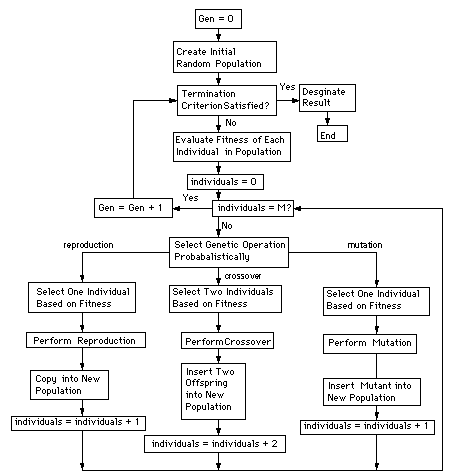
\includegraphics[width=0.8\textwidth]{FlowchartGP.PNG}
  \caption{Diagrama de flujo de la Programación genética.}
  \label{fig:dfd:1}
\end{figure}

\section{Conclusión}

En este trabajo hemos visto desde un punto de vista histórico cómo aparecieron las
metaheurísticas para resolver problemas que resultaban demasiado complejos de resolver
por métodos exactos, por ejemplo, problemas de optimización, ordenación o búsqueda.
Además hemos visto como debido a la falta de medios para comunicarse, aunque con ligeras
diferencias, surgen estrategias muy parecidas, casi al mismo tiempo, como son los algoritmos
genéticos y las estrategias evolutivas en Estados Unidos y Alemania respectivamente, y la importancia
que han tenido en la ciencia de la computación a pesar de que sus comienzos estuvieron
cargados de escepticismo por la falta de una fundamentación teórica que probase su eficacia. \\

Las aplicaciones de estas estrategias son muy extensas como hemos podido ver a lo largo
del trabajo, quedando probada su eficacia con el paso del tiempo y el consecuente aumento
de recursos y capacidad de cómputo. Esto, llevó a que surgiese la programación genética
posteriormente, como una aplicación de los algoritmos genéticos, con la meta de conseguir el
programa mas óptimo para resolver un problema dado de forma automática, además de las futuras
aplicaciones en campos como la computación cuántica.

\section{Referencias}
\begingroup
\renewcommand{\section}[2]{}
\nocite{*}
\printbibliography
\endgroup
\end{document}
